%package list
\documentclass{article}
\usepackage[top=3cm, bottom=3cm, outer=3cm, inner=3cm]{geometry}
\usepackage{multicol}
\usepackage{graphicx}
\usepackage{url}
%\usepackage{cite}
\usepackage{hyperref}
\usepackage{array}
%\usepackage{multicol}
\newcolumntype{x}[1]{>{\centering\arraybackslash\hspace{0pt}}p{#1}}
\usepackage{natbib}
\usepackage{pdfpages}
\usepackage{multirow}
\usepackage[normalem]{ulem}
\useunder{\uline}{\ul}{}
\usepackage{svg}
\usepackage{xcolor}
\usepackage{listings}
\lstdefinestyle{ascii-tree}{
    literate={├}{|}1 {─}{--}1 {└}{+}1 
  }
\lstset{basicstyle=\ttfamily,
  showstringspaces=false,
  commentstyle=\color{red},
  keywordstyle=\color{blue}
}
%\usepackage{booktabs}
\usepackage{caption}
\usepackage{subcaption}
\usepackage{float}
\usepackage{array}
\usepackage{tcolorbox}
\newcolumntype{M}[1]{>{\centering\arraybackslash}m{#1}}
\newcolumntype{N}{@{}m{0pt}@{}}
\usepackage{tabularx}
\usepackage{colortbl}
\usepackage{xcolor}
% \usepackage[margin=1.5cm]{geometry} % Márgenes ajustados
\usepackage{multirow}


%%%%%%%%%%%%%%%%%%%%%%%%%%%%%%%%%%%%%%%%%%%%%%%%%%%%%%%%%%%%%%%%%%%%%%%%%%%%
%%%%%%%%%%%%%%%%%%%%%%%%%%%%%%%%%%%%%%%%%%%%%%%%%%%%%%%%%%%%%%%%%%%%%%%%%%%%
\newcommand{\itemEmail}{rchambillap@unsa.edu.pe}
\newcommand{\itemStudent}{Chambilla Perca, Gutierrez Ccama, Valdivia Segovia}
\newcommand{\itemCourse}{Sistemas Distribuidos}
\newcommand{\itemCourseCode}{}
\newcommand{\itemSemester}{VI}
\newcommand{\itemUniversity}{Universidad Nacional de San Agustín de Arequipa}
\newcommand{\itemFaculty}{Facultad de Ingeniería de Producción y Servicios}
\newcommand{\itemDepartment}{Departamento Académico de Ingeniería de Sistemas e Informática}
\newcommand{\itemSchool}{Escuela Profesional de Ingeniería de Sistemas}
\newcommand{\itemAcademic}{2026 - A}
\newcommand{\itemInput}{Del 20 de Abril 2026}
\newcommand{\itemOutput}{Al 25 de Abril 2026}
\newcommand{\itemPracticeNumber}{02}
\newcommand{\itemTheme}{Sincronización de Relojes: Algoritmos de Cristian y Berkeley}
%%%%%%%%%%%%%%%%%%%%%%%%%%%%%%%%%%%%%%%%%%%%%%%%%%%%%%%%%%%%%%%%%%%%%%%%%%%%
%%%%%%%%%%%%%%%%%%%%%%%%%%%%%%%%%%%%%%%%%%%%%%%%%%%%%%%%%%%%%%%%%%%%%%%%%%%%

\usepackage[english,spanish]{babel}
\usepackage[utf8]{inputenc}
\AtBeginDocument{\selectlanguage{spanish}}
\renewcommand{\figurename}{Figura}
\renewcommand{\refname}{Referencias}
\renewcommand{\tablename}{Tabla} %esto no funciona cuando se usa babel
\AtBeginDocument{%
	\renewcommand\tablename{Tabla}
}

\usepackage{fancyhdr}
\pagestyle{fancy}
\fancyhf{}
\setlength{\headheight}{40.51407pt}
\renewcommand{\headrulewidth}{1pt}
\renewcommand{\footrulewidth}{1pt}
\fancyhead[L]{\raisebox{-0.2\height}{
\includegraphics[width=3cm]{img/logo_episunsa.png}}}
\fancyhead[C]{\fontsize{7}{7}\selectfont	\itemUniversity \\ \itemFaculty \\ \itemDepartment \\ \itemSchool \\ \textbf{\itemCourse}}
\fancyhead[R]{\raisebox{-0.2\height}{
\includegraphics[width=1.2cm]{img/logo_abet.png}}}
\fancyfoot[L]{Grupo Intocables}
\fancyfoot[C]{\itemCourse}
\fancyfoot[R]{Página \thepage}

% para el codigo fuente
\usepackage{listings}
\usepackage{color, colortbl}
\definecolor{dkgreen}{rgb}{0,0.6,0}
\definecolor{gray}{rgb}{0.5,0.5,0.5}
\definecolor{mauve}{rgb}{0.58,0,0.82}
\definecolor{codebackground}{rgb}{0.95, 0.95, 0.92}
\definecolor{tablebackground}{rgb}{0.8, 0, 0}
\definecolor{rojoEncabezado}{HTML}{C0392B} % Color del encabezado
\definecolor{azulDatos}{HTML}{2E5A96}      % Color para el texto en cursiva

\lstset{frame=tb,
	language=Java,
	aboveskip=3mm,
	belowskip=3mm,
	showstringspaces=false,
	columns=flexible,
	basicstyle={\small\ttfamily},
	numbers=left,
	numberstyle=\tiny\color{gray},
	keywordstyle=\color{blue},
	commentstyle=\color{dkgreen},
	stringstyle=\color{mauve},
	breaklines=true,
	breakatwhitespace=true,
	tabsize=3,
	backgroundcolor= \color{codebackground},
}

\begin{document}


	\begin{center}	
		\fontsize{17}{17} \textbf{ Informe de Laboratorio \itemPracticeNumber}
	\end{center}
	\centerline{\textbf{\Large Tema: \itemTheme}}
	
\begin{table}[h]
    \centering
    \renewcommand{\arraystretch}{1.8} % Altura de las filas
    \begin{tabularx}{\textwidth}{|>{\raggedright\arraybackslash\bfseries}p{3.5cm}|X|>{\bfseries}p{2.5cm}|X|>{\bfseries}p{2.5cm}|X|}
        \hline
        % Encabezado principal
        \rowcolor{rojoEncabezado}
        \multicolumn{6}{|c|}{\textcolor{white}{\textbf{INFORMACIÓN BÁSICA}}} \\ \hline
        
        % Asignatura
        ASIGNATURA: & \multicolumn{5}{l|}{SISTEMAS DISTRIBUIDOS} \\ \hline
        
        % Título
        TÍTULO DE LA PRÁCTICA: & \multicolumn{5}{l|}{\textcolor{azulDatos}{\textit{\itemTheme}}} \\ \hline
        
        % Fila de datos numéricos
        NÚMERO DE PRÁCTICA: & \textcolor{azulDatos}{\textit{\itemPracticeNumber}} & AÑO LECTIVO: & 2026 & NRO. SEMESTRE: & 2026A \\ \hline
        
        % Fecha y Hora
        FECHA DE PRESENTACIÓN & \textcolor{azulDatos}{\textit{25/04/2026}} & HORA DE PRESENTACIÓN & \multicolumn{3}{l|}{23:59} \\ \hline
        
        % Integrantes y Nota
        \multicolumn{4}{|l|}{\multirow{2}{*}{\parbox[t]{10cm}{\vspace{0.2cm}\textbf{INTEGRANTE (s): GRUPO `` Intocables ''} \\ \vspace{0.1cm} \quad $\bullet$ CHAMBILLA PERCA RICARDO \\ \quad $\bullet$ JUAN DIEGO GUTIERREZ CCAMA \\ \quad $\bullet$ RYAN FABIAN VALDIVIA SEGOVIA}}} & \multirow{2}{*}{\textbf{NOTA:}} & \multirow{2}{*}{} \\ 
        \multicolumn{4}{|l|}{} & & \\[1cm] \hline
        
        % Docente
        \multicolumn{6}{|l|}{\textbf{DOCENTE(s):}} \\ 
        \multicolumn{6}{|l|}{\textcolor{azulDatos}{\textit{Mg. Maribel Molina Barriga}}} \\ \hline
    \end{tabularx}
\end{table}

	\vspace*{10px}

\section{Repositorio de GitHub y Ejecución}
El código fuente completo de este laboratorio se encuentra alojado en el siguiente repositorio de GitHub: \url{https://github.com/rikich3/LAB_SISTEMAS_DISTRIBUIDOS}

A continuación, se adjunta la captura correspondiente a la ejecución y prueba del ejercicio resuelto sobre el Algoritmo de Lamport:
\begin{figure}[H]
    \centering
    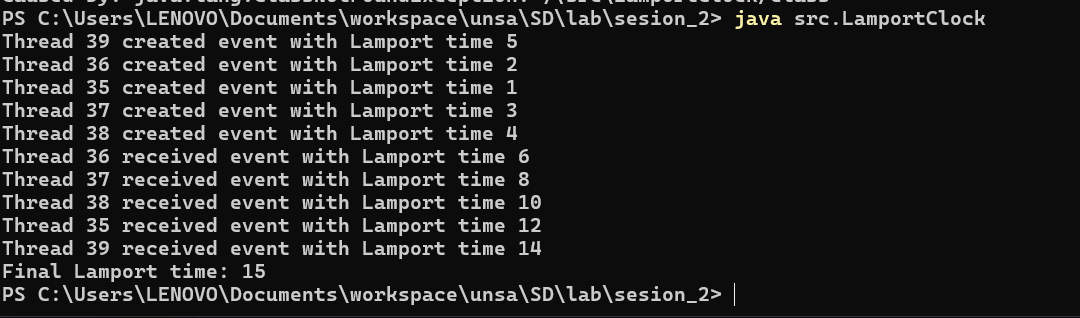
\includegraphics[width=0.85\textwidth]{img/screenshot.png}
    \caption{Ejecución y Prueba del Ejercicio Resuelto: Algoritmo de Lamport}
    \label{fig:lamport_exercise}
\end{figure}

\section{Tareas Realizadas}

Como parte de la sesión de laboratorio 2 de Sistemas Distribuidos, se llevaron a cabo las siguientes tareas:
\begin{itemize}
    \item \textbf{Investigación y Diseño:} Comprensión del funcionamiento interno de ambos algoritmos (Cristian y Berkeley) y cómo simularlos en un entorno local utilizando Java.
    \item \textbf{Implementación mediante Enfoque TDD:} Se escribieron pruebas predefinidas al inicio de cada clase para asegurar el comportamiento correcto (Test-Driven Development) siguiendo las reglas de calidad y metodologías indicadas.
    \item \textbf{Desarrollo del Algoritmo de Cristian (\texttt{CristianAlgorithm.java}):}
    \begin{itemize}
        \item Simula un cliente solicitando el tiempo a un servidor.
        \item Calcula el \textit{Round-Trip Time (RTT)} como la diferencia entre la emisión de la solicitud y la recepción de respuesta.
        \item Ajusta el reloj del cliente en función del tiempo del servidor más la mitad del RTT.
    \end{itemize}
    \item \textbf{Desarrollo del Algoritmo de Berkeley (\texttt{BerkeleyAlgorithm.java}):}
    \begin{itemize}
        \item Simula un demonio o nodo maestro encuestando el estado del tiempo de otros nodos de la red.
        \item Promedia de manera estática los tiempos recolectados.
        \item Retorna un arreglo con los ajustes (deltas) precisos que cada nodo (incluyendo el maestro) debe sumar/restar para sincronizarse exactamente al promedio.
    \end{itemize}
    \item \textbf{Ejecución y Evaluación:} Se compilaron y ejecutaron los algoritmos, validando a través del registro las salidas (logs).
\end{itemize}

\section{Desarrollo de los Ejercicios}

A continuación, se muestra el código fuente de las implementaciones desarrolladas y su correspondiente evaluación.

\subsection{Algoritmo de Cristian}

\lstinputlisting[language=Java, caption={CristianAlgorithm.java: Implementación del Algoritmo de Cristian}]{../src/CristianAlgorithm.java}

\textbf{Ejecución y Resultados:}

Para la ejecución, compilamos y corremos la clase utilizando los siguientes comandos:
\begin{lstlisting}[language=bash, numbers=none, caption={Comandos de compilación y ejecución para Cristian}]
$ javac src/CristianAlgorithm.java
$ java -cp src src.CristianAlgorithm
\end{lstlisting}

\textbf{Salida obtenida:}
\begin{verbatim}
INFO: All tests passed
INFO: Client T0: 1000
INFO: Client T1: 1150
INFO: Server Time returned: 5075
INFO: Calculated RTT: 150
INFO: Synchronized Time: 5150
\end{verbatim}

\textbf{Evaluación:}
El algoritmo logró inferir el retraso introducido por la red (RTT / 2, resultando en 75 ms). Esto permite establecer el reloj local del cliente asumiendo de manera precisa cuánto tiempo transcurrió en el trayecto de vuelta desde el servidor. El enfoque es ideal para tiempos con latencia predecible o que requieran poca sobrecarga en la red.

\subsection{Algoritmo de Berkeley}

\lstinputlisting[language=Java, caption={BerkeleyAlgorithm.java: Implementación del Algoritmo de Berkeley}]{../src/BerkeleyAlgorithm.java}

\textbf{Ejecución y Resultados:}

\begin{lstlisting}[language=bash, numbers=none, caption={Comandos de compilación y ejecución para Berkeley}]
$ javac src/BerkeleyAlgorithm.java
$ java -cp src src.BerkeleyAlgorithm
\end{lstlisting}

\textbf{Salida obtenida:}
\begin{verbatim}
INFO: All tests passed
INFO: Initial Server Time: 3000
INFO: Initial Client Times: [2980, 3015, 3025]
INFO: Adjustments: [5, 25, -10, -20]
INFO: Synchronized Server Time: 3005
INFO: Synchronized Client Times: [3005, 3005, 3005]
\end{verbatim}

\textbf{Evaluación:}
Al calcular el promedio $(3000 + 2980 + 3015 + 3025) / 4 = 3005$, la lógica determinó las distancias exactas que separaban a todos los nodos del equilibrio de la red. Al realizar el ajuste iterativo sobre los relojes, \textbf{todos alcanzaron una sincronización total} al milisegundo ideal (3005 ms). Berkeley demostró ser un método robusto para un entorno distribuido interno donde no se cuente con un receptor de hora externo y asume de manera colaborativa la noción temporal.

\section{Conclusiones}
El uso de TDD y un diseño estricto garantizó implementaciones de alta tolerancia a fallos calculados (las aserciones funcionaron como cortafuegos). Por un lado, el Algoritmo de Cristian nos brinda un modelo más centralizado y simple dependiente de un actor robusto. Por otro, Berkeley resuelve el problema con un enfoque interno en redes locales e interdependientes. La ejecución directa en el espacio de trabajo comprueba que la teoría matemática y de red es correcta.


\clearpage

\section{CUESTIONARIO}

\subsection{1. ¿Por qué es conveniente el uso de relojes lógicos en lugar de los relojes físicos?}
El uso de relojes lógicos es conveniente en un sistema distribuido porque sincronizar relojes físicos de manera exacta es imposible debido a la latencia impredecible de la red y la deriva inherente de los osciladores de cuarzo de cada máquina. En la mayoría de los algoritmos y aplicaciones distribuidas (como bases de datos distribuidas o control de concurrencia), no es necesario conocer la hora exacta real en la que ocurrió un evento, sino el \textbf{orden causal} de los eventos; es decir, qué evento ocurrió antes de otro. Los relojes lógicos, como los de Lamport, garantizan esta relación de orden causal sin requerir de la sincronización de tiempos absolutos complejos y costosos computacionalmente.

\subsection{2. Explique ¿Cuál algoritmo ya sea de Christian o de Berkeley resuelve mejor la sincronización?}
La respuesta depende del contexto y del entorno de red:
\begin{itemize}
    \item \textbf{Algoritmo de Cristian:} Es mejor en entornos donde existe un servidor de tiempo con un reloj de alta precisión (por ejemplo, sincronizado mediante GPS o WWV). Es ideal para redes donde los retrasos de tiempo de ida y vuelta (RTT) son relativamente cortos y estables, ya que compensa la latencia de la red de una manera muy predecible y sencilla.
    \item \textbf{Algoritmo de Berkeley:} Es mejor en un entorno donde \textbf{ninguna de las máquinas cuenta con un receptor de hora exacta}. Este algoritmo funciona buscando que todos los nodos converjan a un tiempo promedio interno y coherente, eliminando los valores atípicos. Esto es especialmente útil en redes aisladas (Intranets cerradas o sistemas embebidos) donde lo que importa es que todos estén de acuerdo en la hora, no que esa hora sea la hora atómica oficial.
\end{itemize}
Por tanto, si se tiene acceso a un servidor con hora exacta, \textbf{Cristian} resuelve el problema de acercarse a la hora real. Si no hay hora real disponible y solo importa la cohesión interna, \textbf{Berkeley} es superior al no depender de un servidor infalible con hardware especial.

\subsection{3. Dado tres procesos P1, P2 y P3, representa la planificación de los procesos siguiendo el algoritmo de ``ocurre antes de''.}
El algoritmo de Lamport basado en "ocurre antes de" ($\rightarrow$) se basa en tres reglas:
\begin{enumerate}
    \item Si dos eventos $a$ y $b$ ocurren en el mismo proceso y $a$ ocurre antes que $b$, entonces $a \rightarrow b$.
    \item Si $a$ es el envío de un mensaje en un proceso y $b$ es la recepción en otro proceso, entonces $a \rightarrow b$.
    \item La relación es transitiva: si $a \rightarrow b$ y $b \rightarrow c$, entonces $a \rightarrow c$.
\end{enumerate}

\textbf{Planificación y Asignación de Tiempos (Ejemplo):}

Supongamos la siguiente interacción entre $P1$, $P2$ y $P3$:
\begin{itemize}
    \item \textbf{P1} genera un evento interno $a$. El reloj de $P1$ avanza a 1: $C(a) = 1$.
    \item \textbf{P1} envía un mensaje $M1$ a $P2$. El evento de envío es $b$. El reloj de $P1$ avanza a 2: $C(b) = 2$. Se adjunta el timestamp 2 al mensaje.
    \item \textbf{P2} tiene un evento interno $c$ (su reloj lógico avanza a 1, $C(c) = 1$).
    \item \textbf{P2} recibe el mensaje $M1$. El evento de recepción es $d$. El reloj de $P2$ se actualiza al máximo entre su reloj local y el tiempo del mensaje + 1: $C(d) = \max(1, 2) + 1 = 3$.
    \item \textbf{P2} envía un mensaje $M2$ a $P3$. El evento de envío es $e$. El reloj avanza a 4: $C(e) = 4$. Se envía con timestamp 4.
    \item \textbf{P3} recibe el mensaje $M2$. El evento de recepción es $f$. Si el reloj local de $P3$ era 0, ahora es $\max(0, 4) + 1 = 5$. $C(f) = 5$.
\end{itemize}
En este escenario, se cumple la relación "ocurre antes de":
$a \rightarrow b \rightarrow d \rightarrow e \rightarrow f$, reflejando que el evento en $P1$ causó en última instancia un evento en $P3$. Los relojes lógicos (1, 2, 3, 4, 5) muestran claramente el orden correcto y causal en el sistema distribuido.

\clearpage
	
	\subsection{\textcolor{red}{Rúbrica para el contenido del Informe y demostración}}
	\begin{itemize}			
		\item El alumno debe marcar o dejar en blanco en celdas de la columna \textbf{Checklist} si cumplio con el ítem correspondiente.
		\item Si un alumno supera la fecha de entrega,  su calificación será sobre la nota mínima aprobada, siempre y cuando cumpla con todos lo items.
		\item El alumno debe autocalificarse en la columna \textbf{Estudiante} de acuerdo a la siguiente tabla:
	
		\begin{table}[ht]
			\caption{Niveles de desempeño}
			\begin{center}
			\begin{tabular}{ccccc}
    			\hline
    			 & \multicolumn{4}{c}{Nivel}\\
    			\cline{1-5}
    			\textbf{Puntos} & Insatisfactorio 25\%& En Proceso 50\% & Satisfactorio 75\% & Sobresaliente 100\%\\
    			\textbf{2.0}&0.5&1.0&1.5&2.0\\
    			\textbf{4.0}&1.0&2.0&3.0&4.0\\
    			\hline
			\end{tabular}
		\end{center}
	\end{table}	
	
	\end{itemize}
	
	\begin{table}[H]
		\caption{Rúbrica para contenido del Informe y demostración}
		\setlength{\tabcolsep}{0.5em} % for the horizontal padding
		{\renewcommand{\arraystretch}{1.5}% for the vertical padding
		%\begin{center}
		\begin{tabular}{|p{2.7cm}|p{7cm}|x{1.3cm}|p{1.2cm}|p{1.5cm}|p{1.1cm}|}
			\hline
    		\multicolumn{2}{|c|}{Contenido y demostración} & Puntos & Checklist & Estudiante & Profesor\\
			\hline
			\textbf{1. GitHub} & Hay enlace URL activo del directorio para el  laboratorio hacia su repositorio GitHub con código fuente terminado y fácil de revisar. &2 &X &2 & \\ 
			\hline
			\textbf{2. Commits} &  Hay capturas de pantalla de los commits más importantes con sus explicaciones detalladas. (El profesor puede preguntar para refrendar calificación). &4 &X &4 & \\ 
			\hline 
			\textbf{3. Código fuente} &  Hay porciones de código fuente importantes con numeración y explicaciones detalladas de sus funciones. &2 &X &2 & \\ 
			\hline 
			\textbf{4. Ejecución} & Se incluyen ejecuciones/pruebas del código fuente  explicadas gradualmente. &2 &X &2 & \\ 
			\hline			
			\textbf{5. Pregunta} & Se responde con completitud a la pregunta formulada en la tarea.  (El profesor puede preguntar para refrendar calificación).  &2 &X &2 & \\ 
			\hline	
			\textbf{6. Fechas} & Las fechas de modificación del código fuente estan dentro de los plazos de fecha de entrega establecidos. &2 &X &2 & \\ 
			\hline 
			\textbf{7. Ortografía} & El documento no muestra errores ortográficos. &2 &X &2 & \\ 
			\hline 
			\textbf{8. Madurez} & El Informe muestra de manera general una evolución de la madurez del código fuente,  explicaciones puntuales pero precisas y un acabado impecable.   (El profesor puede preguntar para refrendar calificación).  &4 &X &4 & \\ 
			\hline
			\multicolumn{2}{|c|}{\textbf{Total}} &20 & &20 & \\ 
			\hline
		\end{tabular}
		%\end{center}
		%\label{tab:multicol}
		}
	\end{table}
	
\clearpage

\section{Referencias}
\begin{itemize}			
	\item Tanenbaum, A.S. (2008). Sistemas distribuidos: principios y paradigmas. México. Pearson Educación.
    \item Ceballos, F. J. (2006). Java 2, Curso de programación. México: Alfaomega, RaMa.
    \item Deitel, H. M., \& Deitel, P. J. (2004). Cómo programar en Java. México: Pearson Educación.
    \item Documentación oficial de Oracle sobre Hilos en Java: \url{https://docs.oracle.com/javase/tutorial/essential/concurrency/index.html}
\end{itemize}	
			
\end{document}